\documentclass[10pt,a4paper]{article}
\usepackage[utf8]{inputenc}
\usepackage[top=2cm,bottom=2cm,left=2cm,right=2cm]{geometry}
\usepackage{amsmath}
\usepackage{amssymb}
\usepackage{array}
\usepackage{tikz}
\usetikzlibrary{arrows.meta,calc,patterns,positioning}
\usepackage{pgfplots}
\pgfplotsset{compat=1.18}
\usepackage[dvipsnames,svgnames]{xcolor}
\usepackage{hyperref}

% Anchor persamaan unik meski nomor di-reset per soal.
\newcounter{eqblock}
\newcommand{\reseteq}{%
  \stepcounter{eqblock}%
  \setcounter{equation}{0}%
  \renewcommand{\theHequation}{\arabic{eqblock}.\arabic{equation}}%
}

\pgfplotsset{
  grafik/.style={
    axis lines=middle,
    xlabel={$x$}, ylabel={$y$},
    width=7.5cm, height=6cm,
    grid=major, grid style={gray!25},
    tick label style={font=\scriptsize},
    every axis x label/.style={at={(ticklabel* cs:1)},anchor=west},
    every axis y label/.style={at={(ticklabel* cs:1)},anchor=south},
    title style={yshift=2ex},
  },
}

\title{Tugas Minggu 4 : Limit}
\author{Matematika untuk Sistem Informasi}
\date{}

\begin{document}

\maketitle

\begin{enumerate}

%===========================================================
\item Hitunglah nilai limit fungsi berikut:
\begin{enumerate}

%-----------------------------------------------------------
\item $\displaystyle\lim_{x \to -1} (1 - 2x)$

\textbf{Jawab:}
\begin{itemize}
\item \textbf{Langkah 1: Kenali Jenis Fungsi}

$1 - 2x$ adalah fungsi linear (polinom), sehingga limitnya dapat dihitung dengan substitusi langsung.

\item \textbf{Langkah 2: Substitusi Langsung}

\reseteq
\begin{align}
\lim_{x \to -1} (1 - 2x) &= 1 - 2(-1) \quad \text{(Substitusi $x = -1$)} \\
&= 1 + 2 = 3
\end{align}
Jadi $\displaystyle\lim_{x \to -1} (1 - 2x) = 3$.
% final: 3
\end{itemize}

%-----------------------------------------------------------
\item $\displaystyle\lim_{t \to 3} \frac{t^2 + 4t - 21}{t - 3}$

\textbf{Jawab:}
\begin{itemize}
\item \textbf{Langkah 1: Coba Substitusi Langsung}

\reseteq
\begin{align}
\frac{3^2 + 4(3) - 21}{3 - 3} &= \frac{9 + 12 - 21}{0} = \frac{0}{0} \quad \text{(Bentuk tak tentu)}
\end{align}

\item \textbf{Langkah 2: Faktorkan dan Sederhanakan}

\reseteq
\begin{align}
\lim_{t \to 3} \frac{t^2 + 4t - 21}{t - 3} &= \lim_{t \to 3} \frac{(t + 7)(t - 3)}{t - 3} \quad \text{(Faktorkan: $7 \cdot (-3) = -21$, $7 + (-3) = 4$)} \\
&= \lim_{t \to 3} (t + 7) \quad \text{(Coret $t - 3$, sah karena $t \neq 3$)}
\end{align}

\item \textbf{Langkah 3: Substitusi Ulang}

\reseteq
\begin{align}
\lim_{t \to 3} (t + 7) &= 3 + 7 = 10
\end{align}
Jadi $\displaystyle\lim_{t \to 3} \frac{t^2 + 4t - 21}{t - 3} = 10$.
% final: 10
\end{itemize}

%-----------------------------------------------------------
\item $\displaystyle\lim_{x \to 9} \frac{x - 9}{\sqrt{x} - 3}$

\textbf{Jawab:}
\begin{itemize}
\item \textbf{Langkah 1: Coba Substitusi Langsung}

\reseteq
\begin{align}
\frac{9 - 9}{\sqrt{9} - 3} &= \frac{0}{3 - 3} = \frac{0}{0} \quad \text{(Bentuk tak tentu)}
\end{align}

\item \textbf{Langkah 2: Kalikan dengan Sekawan Penyebut}

Sekawan dari $\sqrt{x} - 3$ adalah $\sqrt{x} + 3$.
\reseteq
\begin{align}
\lim_{x \to 9} \frac{x - 9}{\sqrt{x} - 3} &= \lim_{x \to 9} \frac{x - 9}{\sqrt{x} - 3} \cdot \frac{\sqrt{x} + 3}{\sqrt{x} + 3} \quad \text{(Kalikan dengan $1$)} \\
&= \lim_{x \to 9} \frac{(x - 9)(\sqrt{x} + 3)}{(\sqrt{x})^2 - 3^2} \quad \text{(Penyebut: $(a-b)(a+b) = a^2 - b^2$)} \\
&= \lim_{x \to 9} \frac{(x - 9)(\sqrt{x} + 3)}{x - 9} \quad \text{(Sederhanakan penyebut)} \\
&= \lim_{x \to 9} (\sqrt{x} + 3) \quad \text{(Coret $x - 9$, sah karena $x \neq 9$)}
\end{align}

\item \textbf{Langkah 3: Substitusi Ulang}

\reseteq
\begin{align}
\lim_{x \to 9} (\sqrt{x} + 3) &= \sqrt{9} + 3 = 3 + 3 = 6
\end{align}
Jadi $\displaystyle\lim_{x \to 9} \frac{x - 9}{\sqrt{x} - 3} = 6$.
% final: 6
\end{itemize}

\end{enumerate}

%===========================================================
\item Diberikan grafik fungsi berikut:

\begin{center}
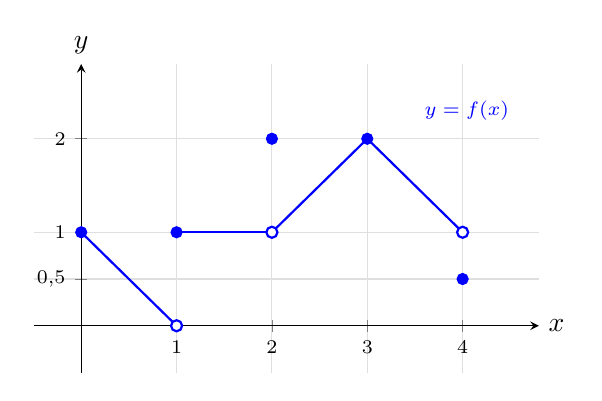
\begin{tikzpicture}
\begin{axis}[grafik, width=8cm, height=5.5cm, xmin=-0.5, xmax=4.8, ymin=-0.5, ymax=2.8,
  xtick={1,2,3,4}, ytick={0.5,1,2}, yticklabels={$0{,}5$,$1$,$2$}]
  \addplot[thick, blue, no marks] coordinates {(0,1) (1,0)};
  \addplot[thick, blue, no marks] coordinates {(1,1) (2,1)};
  \addplot[thick, blue, no marks] coordinates {(2,1) (3,2) (4,1)};
  \filldraw[blue] (axis cs:0,1) circle (2pt);
  \filldraw[blue, fill=white, thick] (axis cs:1,0) circle (2pt);
  \filldraw[blue] (axis cs:1,1) circle (2pt);
  \filldraw[blue, fill=white, thick] (axis cs:2,1) circle (2pt);
  \filldraw[blue] (axis cs:2,2) circle (2pt);
  \filldraw[blue] (axis cs:3,2) circle (2pt);
  \filldraw[blue, fill=white, thick] (axis cs:4,1) circle (2pt);
  \filldraw[blue] (axis cs:4,0.5) circle (2pt);
  \node[blue, font=\scriptsize, anchor=west] at (axis cs:3.5,2.3) {$y = f(x)$};
\end{axis}
\end{tikzpicture}
\end{center}

Cari limit/nilai fungsi berikut, atau nyatakan bahwa limit/nilai fungsi tidak ada.

\begin{center}
\begin{tabular}{llll}
(a) $\displaystyle\lim_{x \to 1^-} f(x)$ & (b) $\displaystyle\lim_{x \to 1^+} f(x)$ & (c) $\displaystyle\lim_{x \to 2} f(x)$ & (d) $\displaystyle\lim_{x \to 3} f(x)$ \\[3ex]
(e) $\displaystyle\lim_{x \to 1} f(x)$ & (f) $f(2)$ & (g) $f(3)$ & (h) $f(4)$
\end{tabular}
\end{center}

\textbf{Jawab:}
\begin{itemize}
\item \textbf{Langkah 1: Bedakan Limit dan Nilai Fungsi}

Limit dibaca dari ke mana \emph{kurva} menuju ketika $x$ mendekati titik tersebut; nilai fungsi dibaca dari \emph{titik penuh} ($\bullet$) tepat di atas titik tersebut. Titik kosong ($\circ$) bukan nilai fungsi.
Dari grafik, aturan fungsi dapat ditulis sebagai
\[
f(x) =
\begin{cases}
  -x + 1, & 0 \le x < 1 \\
  1, & 1 \le x < 2 \\
  2, & x = 2 \\
  x - 1, & 2 < x \le 3 \\
  -x + 5, & 3 < x < 4 \\
  0{,}5, & x = 4
\end{cases}
\]

\item \textbf{Langkah 2: Baca Limit}

\begin{enumerate}
  \item[(a)] Dari kiri $x = 1$, kurva $y = -x + 1$ menuju titik kosong $(1,0)$:
  \reseteq
  \begin{align}
  \lim_{x \to 1^-} f(x) &= \lim_{x \to 1^-} (-x + 1) = -1 + 1 = 0 \quad \text{(Aturan untuk $0 \le x < 1$)}
  \end{align}
  % final: 0
  \item[(b)] Dari kanan $x = 1$, kurva mendatar $y = 1$ menuju titik penuh $(1,1)$:
  \reseteq
  \begin{align}
  \lim_{x \to 1^+} f(x) &= \lim_{x \to 1^+} 1 = 1 \quad \text{(Aturan untuk $1 \le x < 2$)}
  \end{align}
  % final: 1
  \item[(c)] Aturan fungsi berubah di $x = 2$, sehingga dihitung limit kiri dan limit kanan:
  \reseteq
  \begin{align}
  \lim_{x \to 2^-} f(x) &= \lim_{x \to 2^-} 1 = 1 \quad \text{(Aturan untuk $1 \le x < 2$)} \\
  \lim_{x \to 2^+} f(x) &= \lim_{x \to 2^+} (x - 1) = 2 - 1 = 1 \quad \text{(Aturan untuk $2 < x \le 3$)}
  \end{align}
  Kedua arah menuju titik kosong $(2,1)$, jadi $\displaystyle\lim_{x \to 2} f(x) = 1$.
  % final: 1
  \item[(d)] Aturan fungsi juga berubah di $x = 3$:
  \reseteq
  \begin{align}
  \lim_{x \to 3^-} f(x) &= \lim_{x \to 3^-} (x - 1) = 3 - 1 = 2 \quad \text{(Aturan untuk $2 < x \le 3$)} \\
  \lim_{x \to 3^+} f(x) &= \lim_{x \to 3^+} (-x + 5) = -3 + 5 = 2 \quad \text{(Aturan untuk $3 < x < 4$)}
  \end{align}
  Kedua arah menuju titik puncak $(3,2)$, jadi $\displaystyle\lim_{x \to 3} f(x) = 2$.
  % final: 2
  \item[(e)] Karena $\displaystyle\lim_{x \to 1^-} f(x) = 0 \neq 1 = \lim_{x \to 1^+} f(x)$, maka $\displaystyle\lim_{x \to 1} f(x)$ \textbf{tidak ada}.
  % final: \text{tidak ada}
\end{enumerate}

\item \textbf{Langkah 3: Baca Nilai Fungsi}

\begin{enumerate}
  \item[(f)] Titik penuh di $x = 2$ adalah $(2,2)$, jadi $f(2) = 2$. Perhatikan bahwa $f(2) = 2$ berbeda dengan $\lim_{x \to 2} f(x) = 1$.
  % final: 2
  \item[(g)] Titik penuh di $x = 3$ adalah $(3,2)$, jadi $f(3) = 2$, sama dengan $\lim_{x \to 3} f(x)$.
  % final: 2
  \item[(h)] Titik penuh di $x = 4$ adalah $(4, 0{,}5)$, jadi $f(4) = 0{,}5$. Titik $(4,1)$ kosong, sehingga bukan nilai $f(4)$.
  % final: 0{,}5
\end{enumerate}
\end{itemize}

%===========================================================
\item Diketahui
\[
f(x) =
\begin{cases}
  x^2 + 1, & x \le 1 \\
  x^2 - x + 2, & x > 1
\end{cases}
\]
\begin{enumerate}

%-----------------------------------------------------------
\item Hitung $\displaystyle\lim_{x \to 1^-} f(x)$ dan $\displaystyle\lim_{x \to 1^+} f(x)$.

\textbf{Jawab:}
\begin{itemize}
\item \textbf{Langkah 1: Tentukan Titik Perubahan Aturan}

Aturan fungsi berubah di $x = 1$: untuk $x < 1$ berlaku $f(x) = x^2 + 1$, dan untuk $x > 1$ berlaku $f(x) = x^2 - x + 2$.

\item \textbf{Langkah 2: Hitung Limit Kiri dan Limit Kanan}

\reseteq
\begin{align}
\lim_{x \to 1^-} f(x) &= \lim_{x \to 1^-} (x^2 + 1) = 1^2 + 1 = 2 \quad \text{(Aturan untuk $x < 1$)} \\
\lim_{x \to 1^+} f(x) &= \lim_{x \to 1^+} (x^2 - x + 2) = 1^2 - 1 + 2 = 2 \quad \text{(Aturan untuk $x > 1$)}
\end{align}
Jadi $\displaystyle\lim_{x \to 1^-} f(x) = 2$ dan $\displaystyle\lim_{x \to 1^+} f(x) = 2$.
% final: 2
\end{itemize}

%-----------------------------------------------------------
\item Selidiki apakah $\displaystyle\lim_{x \to 1} f(x)$ ada, jika ada hitung limitnya.

\textbf{Jawab:}
\begin{itemize}
\item \textbf{Langkah 1: Gunakan Teorema Keberadaan Limit}

$\displaystyle\lim_{x \to 1} f(x)$ ada jika dan hanya jika limit kiri sama dengan limit kanan. Dari bagian (a),
\[
\lim_{x \to 1^-} f(x) = 2 = \lim_{x \to 1^+} f(x).
\]
Jadi $\displaystyle\lim_{x \to 1} f(x)$ \textbf{ada} dan $\displaystyle\lim_{x \to 1} f(x) = 2$.
% final: 2

\item \textbf{Langkah 2: Verifikasi dengan Grafik}

\begin{center}
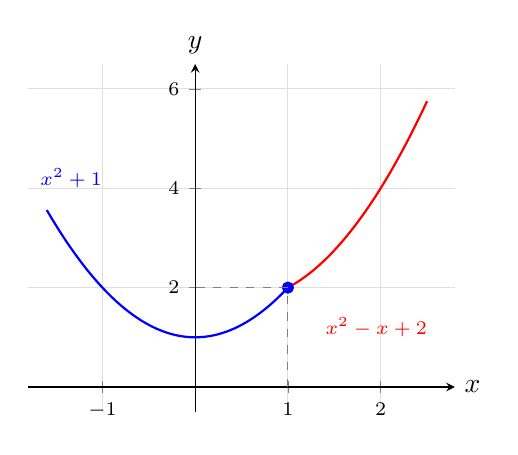
\begin{tikzpicture}
\begin{axis}[grafik, width=7cm, height=6cm, xmin=-1.8, xmax=2.8, ymin=-0.5, ymax=6.5]
  \addplot[domain=-1.6:1, samples=60, thick, blue] {x^2 + 1};
  \addplot[domain=1:2.5, samples=60, thick, Red] {x^2 - x + 2};
  \filldraw[blue] (axis cs:1,2) circle (2pt);
  \draw[dashed, gray] (axis cs:1,0) -- (axis cs:1,2) -- (axis cs:0,2);
  \node[font=\scriptsize, blue, anchor=east] at (axis cs:-0.9,4.2) {$x^2 + 1$};
  \node[font=\scriptsize, Red, anchor=west] at (axis cs:1.3,1.2) {$x^2 - x + 2$};
\end{axis}
\end{tikzpicture}
\end{center}
Kedua potongan bersambung di titik $(1,2)$, sesuai dengan $\displaystyle\lim_{x \to 1} f(x) = 2$.
\end{itemize}

\end{enumerate}

%===========================================================
\item Hitunglah nilai limit trigonometri berikut ini:
\begin{enumerate}

%-----------------------------------------------------------
\item $\displaystyle\lim_{t \to 0} \frac{\sin 3t}{\tan t}$

\textbf{Jawab:}
\begin{itemize}
\item \textbf{Langkah 1: Coba Substitusi Langsung}

$\dfrac{\sin 0}{\tan 0} = \dfrac{0}{0}$, bentuk tak tentu.

\item \textbf{Langkah 2: Bentuk Pola Dasar}

\reseteq
\begin{align}
\lim_{t \to 0} \frac{\sin 3t}{\tan t} &= \lim_{t \to 0} \frac{\frac{\sin 3t}{3t} \cdot 3t}{\frac{\tan t}{t} \cdot t} \quad \text{(Kalikan dan bagi dengan $3t$ dan $t$)} \\
&= \lim_{t \to 0} \frac{\frac{\sin 3t}{3t}}{\frac{\tan t}{t}} \cdot 3 \quad \text{(Coret $t$)} \\
&= \frac{1}{1} \cdot 3 = 3 \quad \text{(Limit dasar)}
\end{align}
Jadi $\displaystyle\lim_{t \to 0} \frac{\sin 3t}{\tan t} = 3$, sesuai bentuk umum $\frac{a}{b} = \frac{3}{1}$.
% final: 3
\end{itemize}

%-----------------------------------------------------------
\item $\displaystyle\lim_{t \to 0} \frac{\sin^2 3t}{2t^2}$

\textbf{Jawab:}
\begin{itemize}
\item \textbf{Langkah 1: Coba Substitusi Langsung}

$\dfrac{\sin^2 0}{2 \cdot 0^2} = \dfrac{0}{0}$, bentuk tak tentu.

\item \textbf{Langkah 2: Bentuk Pola Dasar}

\reseteq
\begin{align}
\lim_{t \to 0} \frac{\sin^2 3t}{2t^2} &= \lim_{t \to 0} \frac{1}{2} \cdot \frac{\sin 3t}{t} \cdot \frac{\sin 3t}{t} \quad \text{(Pecah $\sin^2 3t = \sin 3t \cdot \sin 3t$)} \\
&= \lim_{t \to 0} \frac{1}{2} \cdot 3 \cdot \frac{\sin 3t}{3t} \cdot 3 \cdot \frac{\sin 3t}{3t} \quad \text{(Bentuk pola $\tfrac{\sin 3t}{3t}$)} \\
&= \frac{9}{2} \cdot \left(\lim_{t \to 0} \frac{\sin 3t}{3t}\right)^2 \quad \text{(Sifat hasil kali)} \\
&= \frac{9}{2} \cdot 1^2 = \frac{9}{2} \quad \text{(Limit dasar)}
\end{align}
Jadi $\displaystyle\lim_{t \to 0} \frac{\sin^2 3t}{2t^2} = \frac{9}{2}$.
% final: \frac{9}{2}
\end{itemize}

%-----------------------------------------------------------
\item $\displaystyle\lim_{x \to 0} \frac{3x \tan x}{\sin x}$

\textbf{Jawab:}
\begin{itemize}
\item \textbf{Langkah 1: Coba Substitusi Langsung}

$\dfrac{3 \cdot 0 \cdot \tan 0}{\sin 0} = \dfrac{0}{0}$, bentuk tak tentu.

\item \textbf{Langkah 2: Sederhanakan dengan Identitas}

\reseteq
\begin{align}
\frac{3x \tan x}{\sin x} &= \frac{3x \cdot \frac{\sin x}{\cos x}}{\sin x} \quad \text{(Identitas $\tan x = \tfrac{\sin x}{\cos x}$)} \\
&= \frac{3x}{\cos x} \quad \text{(Coret $\sin x$, sah karena $\sin x \neq 0$ untuk $x$ dekat $0$, $x \neq 0$)}
\end{align}

\item \textbf{Langkah 3: Substitusi Ulang}

\reseteq
\begin{align}
\lim_{x \to 0} \frac{3x \tan x}{\sin x} &= \lim_{x \to 0} \frac{3x}{\cos x} = \frac{3 \cdot 0}{\cos 0} = \frac{0}{1} = 0
\end{align}
Jadi $\displaystyle\lim_{x \to 0} \frac{3x \tan x}{\sin x} = 0$.
% final: 0
\end{itemize}

\end{enumerate}

%===========================================================
\item Hitung nilai limit berikut:
\begin{enumerate}

%-----------------------------------------------------------
\item $\displaystyle\lim_{n \to \infty} \frac{n^2}{2n + 1}$

\textbf{Jawab:}
\begin{itemize}
\item \textbf{Langkah 1: Bandingkan Derajat}

Derajat pembilang ($2$) lebih besar dari derajat penyebut ($1$), sehingga limitnya tak hingga.

\item \textbf{Langkah 2: Bagi dengan $n$ (Pangkat Tertinggi Penyebut)}

\reseteq
\begin{align}
\lim_{n \to \infty} \frac{n^2}{2n + 1} &= \lim_{n \to \infty} \frac{\frac{n^2}{n}}{\frac{2n}{n} + \frac{1}{n}} \quad \text{(Bagi setiap suku dengan $n$)} \\
&= \lim_{n \to \infty} \frac{n}{2 + \frac{1}{n}} \\
&= \infty \quad \text{(Pembilang $n \to \infty$, penyebut $2 + \tfrac{1}{n} \to 2$)}
\end{align}
Jadi $\displaystyle\lim_{n \to \infty} \frac{n^2}{2n + 1} = +\infty$, artinya nilai $\frac{n^2}{2n+1}$ membesar tanpa batas; limit ini tidak ada sebagai bilangan real.
% final: \infty
\end{itemize}

%-----------------------------------------------------------
\item $\displaystyle\lim_{n \to \infty} \frac{3n^2}{2n^2 + 1}$

\textbf{Jawab:}
\begin{itemize}
\item \textbf{Langkah 1: Bandingkan Derajat}

Derajat pembilang dan penyebut sama (keduanya $2$), dengan koefisien utama $a_2 = 3$ dan $b_2 = 2$, sehingga limitnya diharapkan $\frac{3}{2}$.

\item \textbf{Langkah 2: Bagi dengan $n^2$}

\reseteq
\begin{align}
\lim_{n \to \infty} \frac{3n^2}{2n^2 + 1} &= \lim_{n \to \infty} \frac{\frac{3n^2}{n^2}}{\frac{2n^2}{n^2} + \frac{1}{n^2}} \quad \text{(Bagi setiap suku dengan $n^2$)} \\
&= \lim_{n \to \infty} \frac{3}{2 + \frac{1}{n^2}} = \frac{3}{2 + 0} = \frac{3}{2} \quad \text{(Gunakan $\tfrac{a}{n^k} \to 0$)}
\end{align}
Jadi $\displaystyle\lim_{n \to \infty} \frac{3n^2}{2n^2 + 1} = \frac{3}{2}$.
% final: \frac{3}{2}
\end{itemize}

%-----------------------------------------------------------
\item $\displaystyle\lim_{x \to \infty} \frac{x}{1 + x^2}$

\textbf{Jawab:}
\begin{itemize}
\item \textbf{Langkah 1: Bandingkan Derajat}

Derajat pembilang $n = 1$ lebih kecil dari derajat penyebut $m = 2$, sehingga limitnya diharapkan $0$.

\item \textbf{Langkah 2: Bagi dengan $x^2$}

\reseteq
\begin{align}
\lim_{x \to \infty} \frac{x}{1 + x^2} &= \lim_{x \to \infty} \frac{\frac{x}{x^2}}{\frac{1}{x^2} + \frac{x^2}{x^2}} \quad \text{(Bagi setiap suku dengan $x^2$)} \\
&= \lim_{x \to \infty} \frac{\frac{1}{x}}{\frac{1}{x^2} + 1} = \frac{0}{0 + 1} = 0 \quad \text{(Gunakan $\tfrac{a}{x^k} \to 0$)}
\end{align}
Jadi $\displaystyle\lim_{x \to \infty} \frac{x}{1 + x^2} = 0$.
% final: 0
\end{itemize}

\end{enumerate}

\end{enumerate}

\end{document}
